\chapter{Představení problematiky detekce pádu}
\label{chap:Goal}

V této kapitole je stanoven přesný cíl a navržen postup, jak k problému
přistoupit.

Úkolem bude v reálném čase z videostreamu detekovat pád osoby. Pád osoby
je definován jako náhlé, neúmyslné klesnutí těla z výškové pozice (např. stání,
chůze nebo sezení) na zem nebo jinou nižší úroveň, přičemž tato osoba nemá
kontrolu nad tímto pohybem. Samozřejmě není vždy možné úplně dobře
rozeznat, zda se nejedná o úmyslné klesnutí, např. prudké lehnutí.

Dle některých definic (zejména ve zdravotnictví) se o pád nejedná, pokud jde o
důsledek závažné vnitřní příhody (např. mrtvice). Toto zde nebude rozlišováno,
naopak bude cílem detekovat jak pády v důsledku ztráty rovnováhy či vlivem
vnějších faktorů (např. zakopnutí, převrácení těžkým předmětem), tak pády v
důsledku akutních události vlivem zdravotních problémů, jako jsou např.
mrtvice, záchvaty, mdloby či jiné důvody ztráty vědomí.

\section{Návrh řešení}

Cílem této práce je navrhnout algoritmus, který bude detekovat, zda je ve
vstupní sekvenci snímku nějaká osoba, jejíž pozice je klasifikována jako pád.
Hlavním cílem výsledného programu bude alarmovat příslušného pracovníka, pokud
osoba upadne.

Alarmovat se bude až tehdy, když osoba zůstane v ležící pozici. To umožní
odfiltrovat falešné alarmy v případě sehnutí či pokud bude osoba špatně
viditelná a algoritmus tak na okamžik špatně vyhodnotí její pohyb. Tímto
postprocesingem se ale práce nebude zabývat, pozornost bude věnována spíše
samotné klasifikaci pozice.

Stejně jako u detekce objektů, viz \ref{sec:obj_det}, by bylo možné i pro
detekci pádu vytvořit vhodnou konvoluční síť, která by přímo z obrázku
definovala, zda se jedná o pád nebo ne. U detekce se už dnes sice s ohledem na
pokrok hardwaru tento přístup používá, nicméně se jedná o velmi náročný úkol,
který vyžaduje rozsáhlou optimalizaci, pokročilou architekturu a velké množství
trénovacích dat. Nicméně, pokud by se podařilo takovouto síť natrénovat, mohla
by lépe detekovat některé situace např. podle výrazu tváře.

V navrženém řešení tedy bude v prvním kroku pomocí vhodné předtrénované
neuronové sítě detekována pozice osoby ve formě klíčových bodů, tato část bude
nazývána \textit{detekční algoritmus}. Na základě těchto bodů pak další
neuronová síť vyhodnotí, zda se jedná o pád, tato část bude nazývána
\textit{klasifikační algoritmus}. To úlohu velice zjednoduší, jelikož místo
analyzování tisíců pixelů, bude algoritmus analyzovat pár desítek klíčových
bodů. Další výhodou je, že u takového postupu je možné použít techniky, kdy je
sledována změna pózy v čase, což by bylo mnohem složitější s jednofázovou
konvoluční síti.

Detekční algoritmus dostane na vstup celý snímek a může detekovat několik osob.
Klasifikační algoritmus ale bude zpracovávat každou osobu, resp. její pózu,
zvlášť.

Další alternativou by mohlo být pouze detekovat osoby jako objekty, a na
základě jejich bounding boxů určit, zda se jedná o pád. Tento postup by byl
jednodušší na dvou úrovních. Jednak je detekce objektů méně náročná úloha než
detekce pózy, jednak by ve druhé fázi bylo analyzováno pouze několik parametrů
bounding boxu (rozměry a velikost) oproti pár desítkám klíčových bodů. Hlubší úvaha však napoví, že parametry bounding boxů ne vždy vypovídají o pozici
člověka. Tento postup by tak pravděpodobně vedl k mnohem méně přesnému
výsledku, než analýza klíčových bodů, kdy může síť analyzovat takové vzorce
jako je např. délka končetin v pohledu či úhel mezi nimi.

Nyní bude popsáno, jak a z jakými daty se bude pracovat, zejména při trénování,
v další kapitole pak bude rozebrána problematika detekce pózy a bude zvolen
algoritmus pro detekci klíčových bodů. Dále se bude práce věnovat vývoji modelu
detekujícího pád na základě těchto klíčových bodů.

\section{Trénovací datasety}
\label{sec:TrainingData}

Pro trénování vyvíjeného modelu bylo použito necelých 150 krátkých (1 až 15
sekund) videí ze dvou zdrojů. Prvním je dataset CAUCAFall vytvořený právě pro
práci s pády osob \cite{caucafall}. Tento dataset obsahuje 100 nahrávek
simulovaných pádů v různých světelných podmínkách, s různými osobami. Zahrnují
širokou škálu scénářů, jednak pro různé druhy pádů (v různých směrech či z
židle), jednak pro situace podobné pádu, jako je kleknutí či sehnutí se, jednak
běžné činnosti jako chůze či sednutí. Poměr videí s úpadkem a bez je 50/50.

Dalším zdrojem pro trénovací data je YouTube video tvůrce Kevina Parryho
\textit{50 Ways to Fall}. Ve videu autor simuluje pády v různých scénářích,
jako je zakopnutí, omdlení či poražení elektrickým proudem. Vzhledem k zabavné
povaze videa byly některé scénáře vypuštěny, nakonec bylo použito 45 videí. Zde
prakticky všechny videa obsahují pád, v některých se ale postava vrátí do
normálního stavu (např. kotrmelec).

\begin{figure}[]
    \centering
    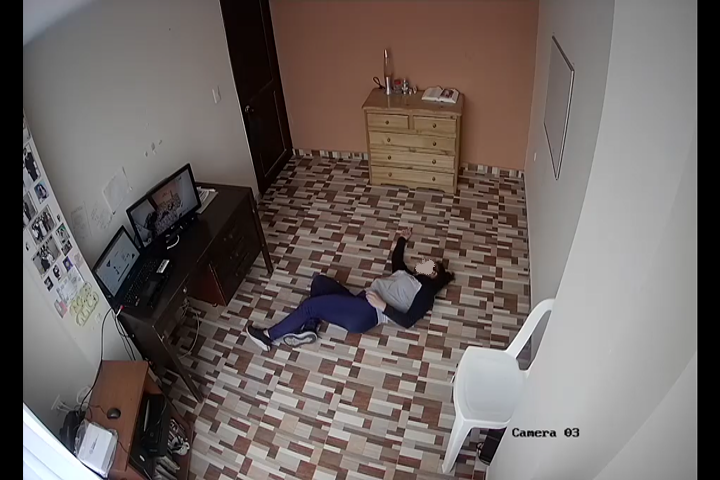
\includegraphics[width=0.45\textwidth]{Figures/datasets_examples/cauca1.png}
    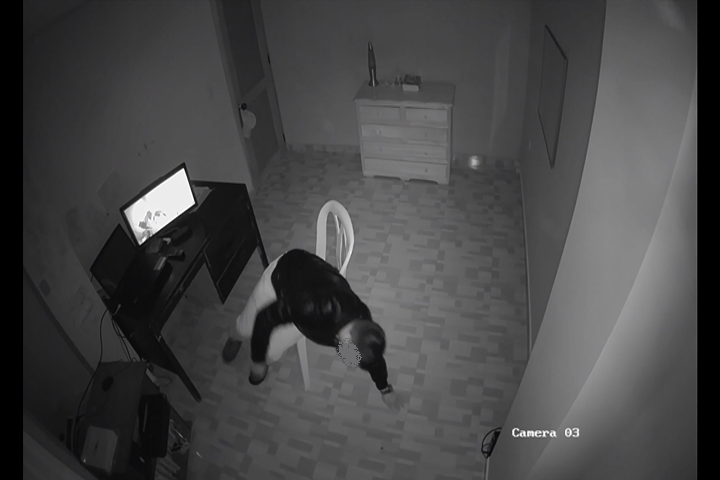
\includegraphics[width=0.45\textwidth]{Figures/datasets_examples/cauca2.png}
    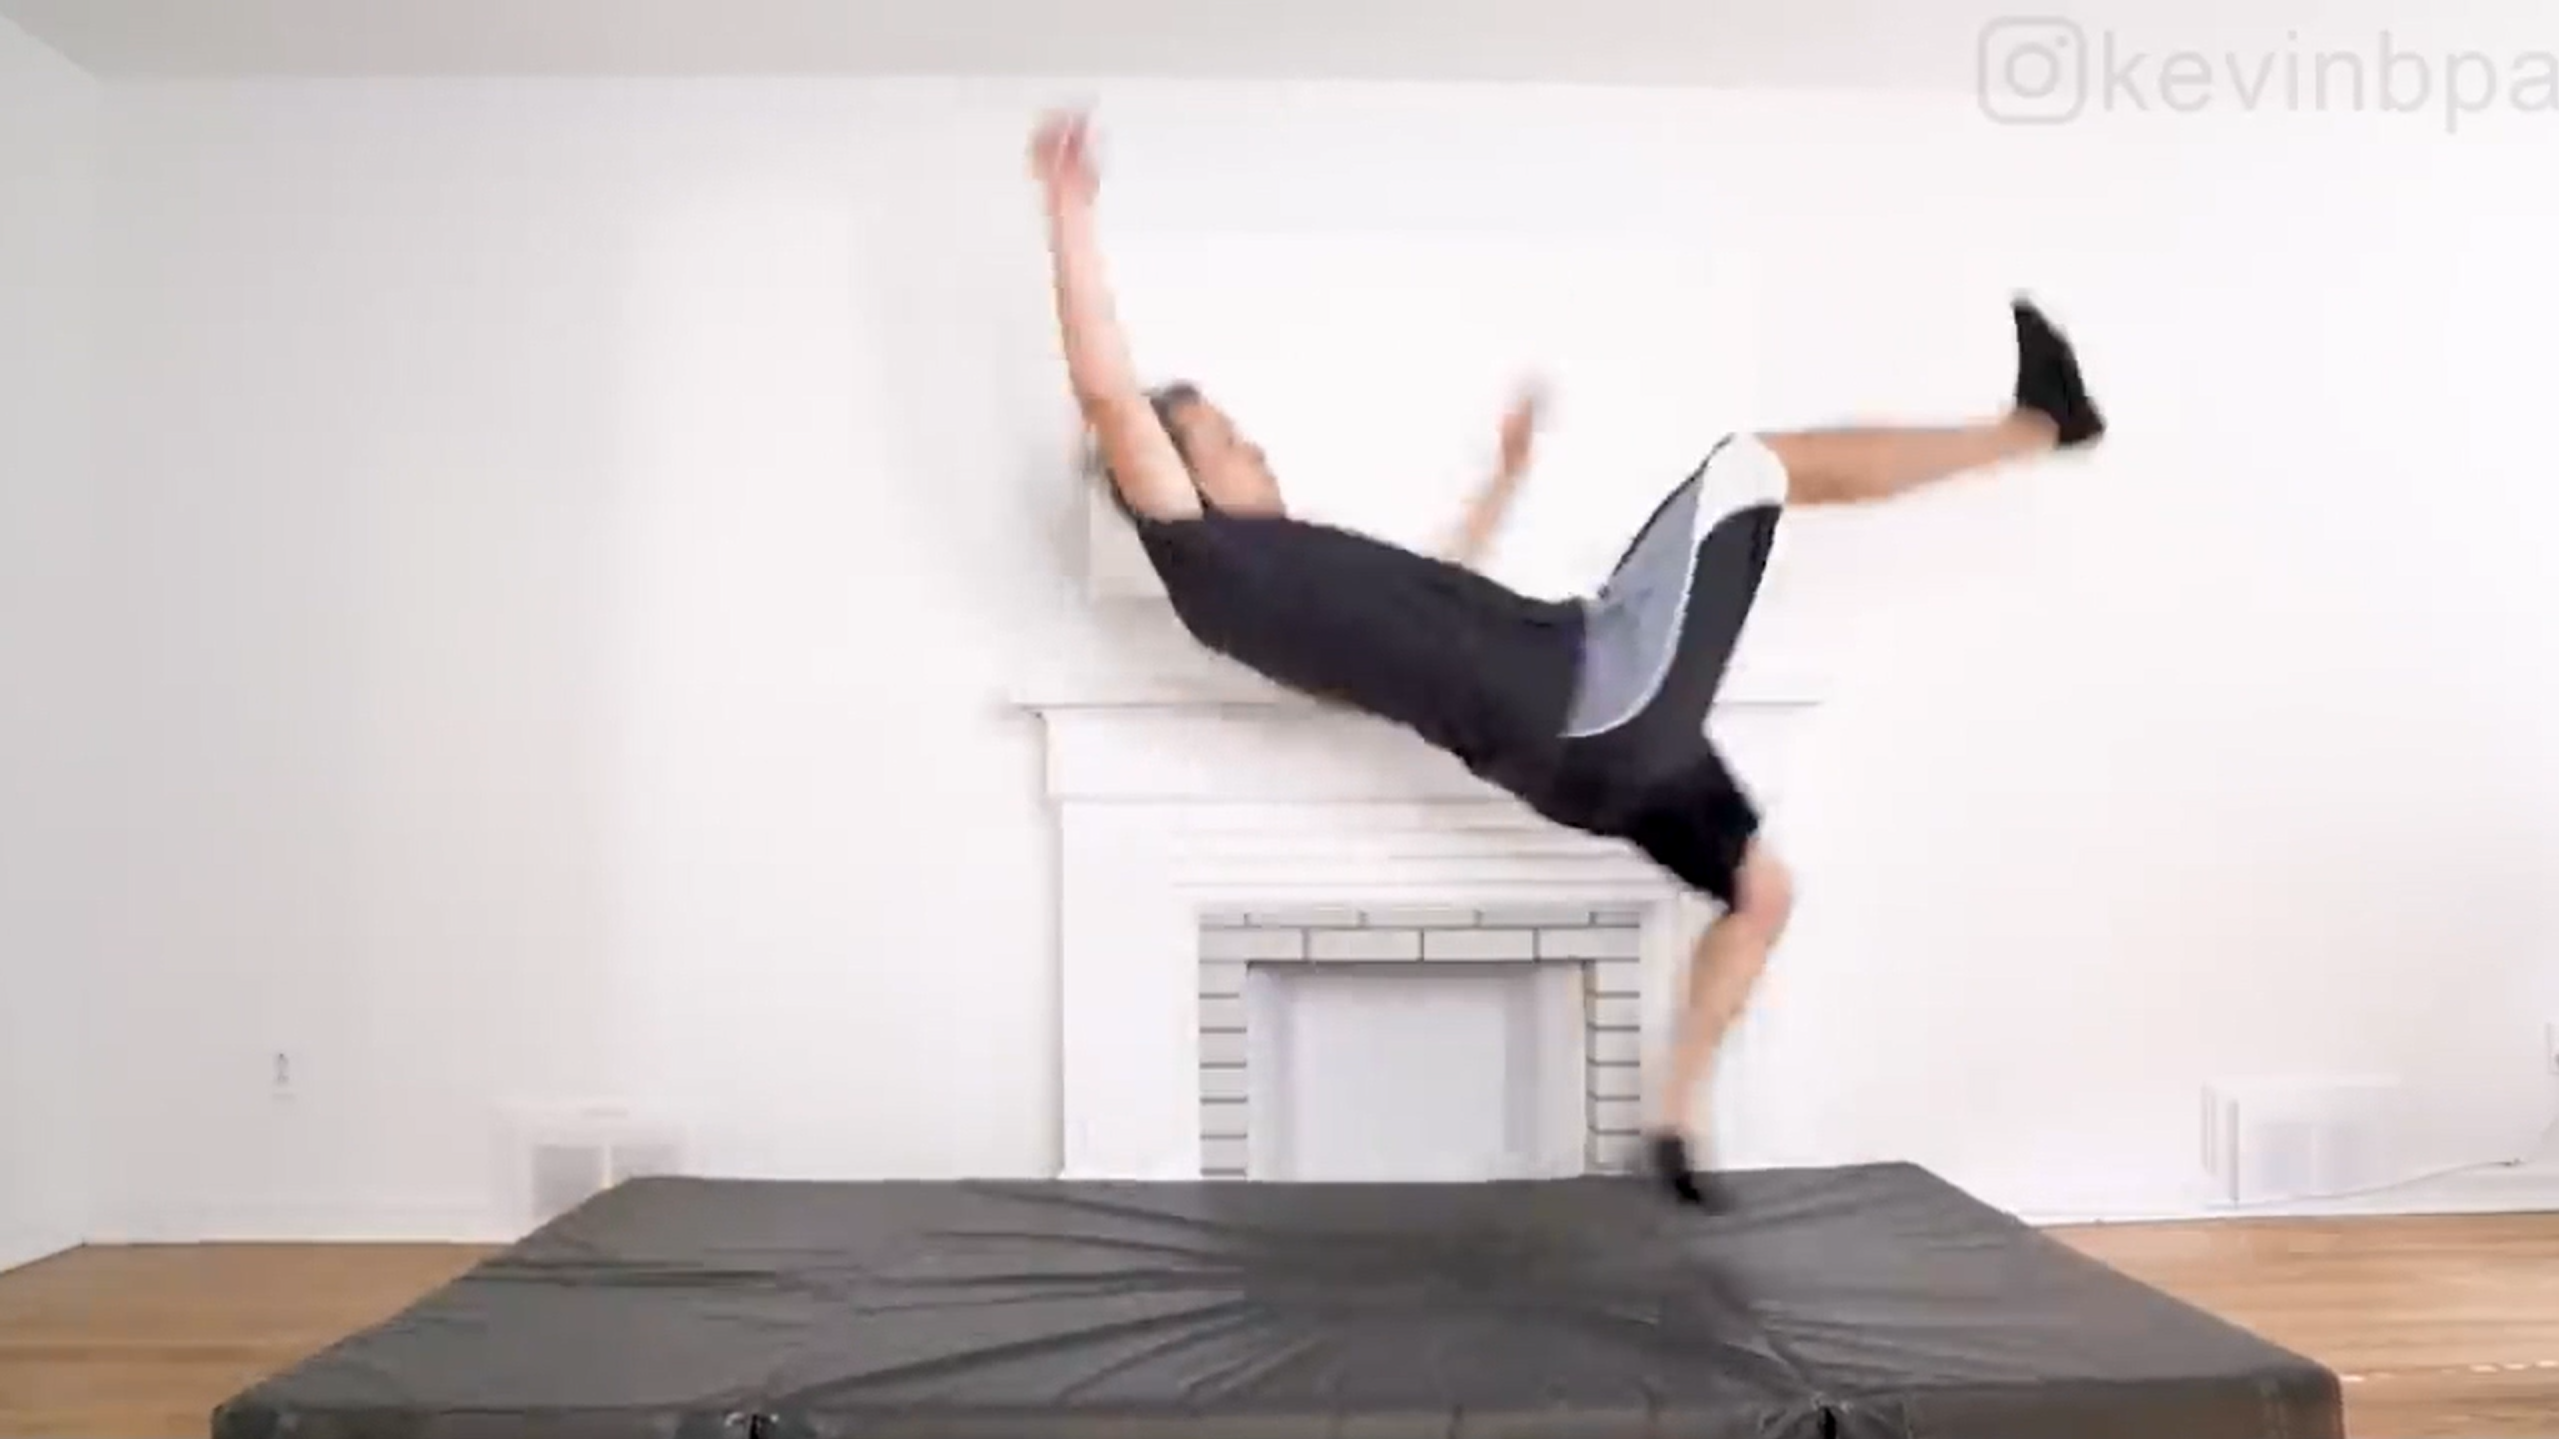
\includegraphics[width=0.45\textwidth]{Figures/datasets_examples/fifty1.png}
    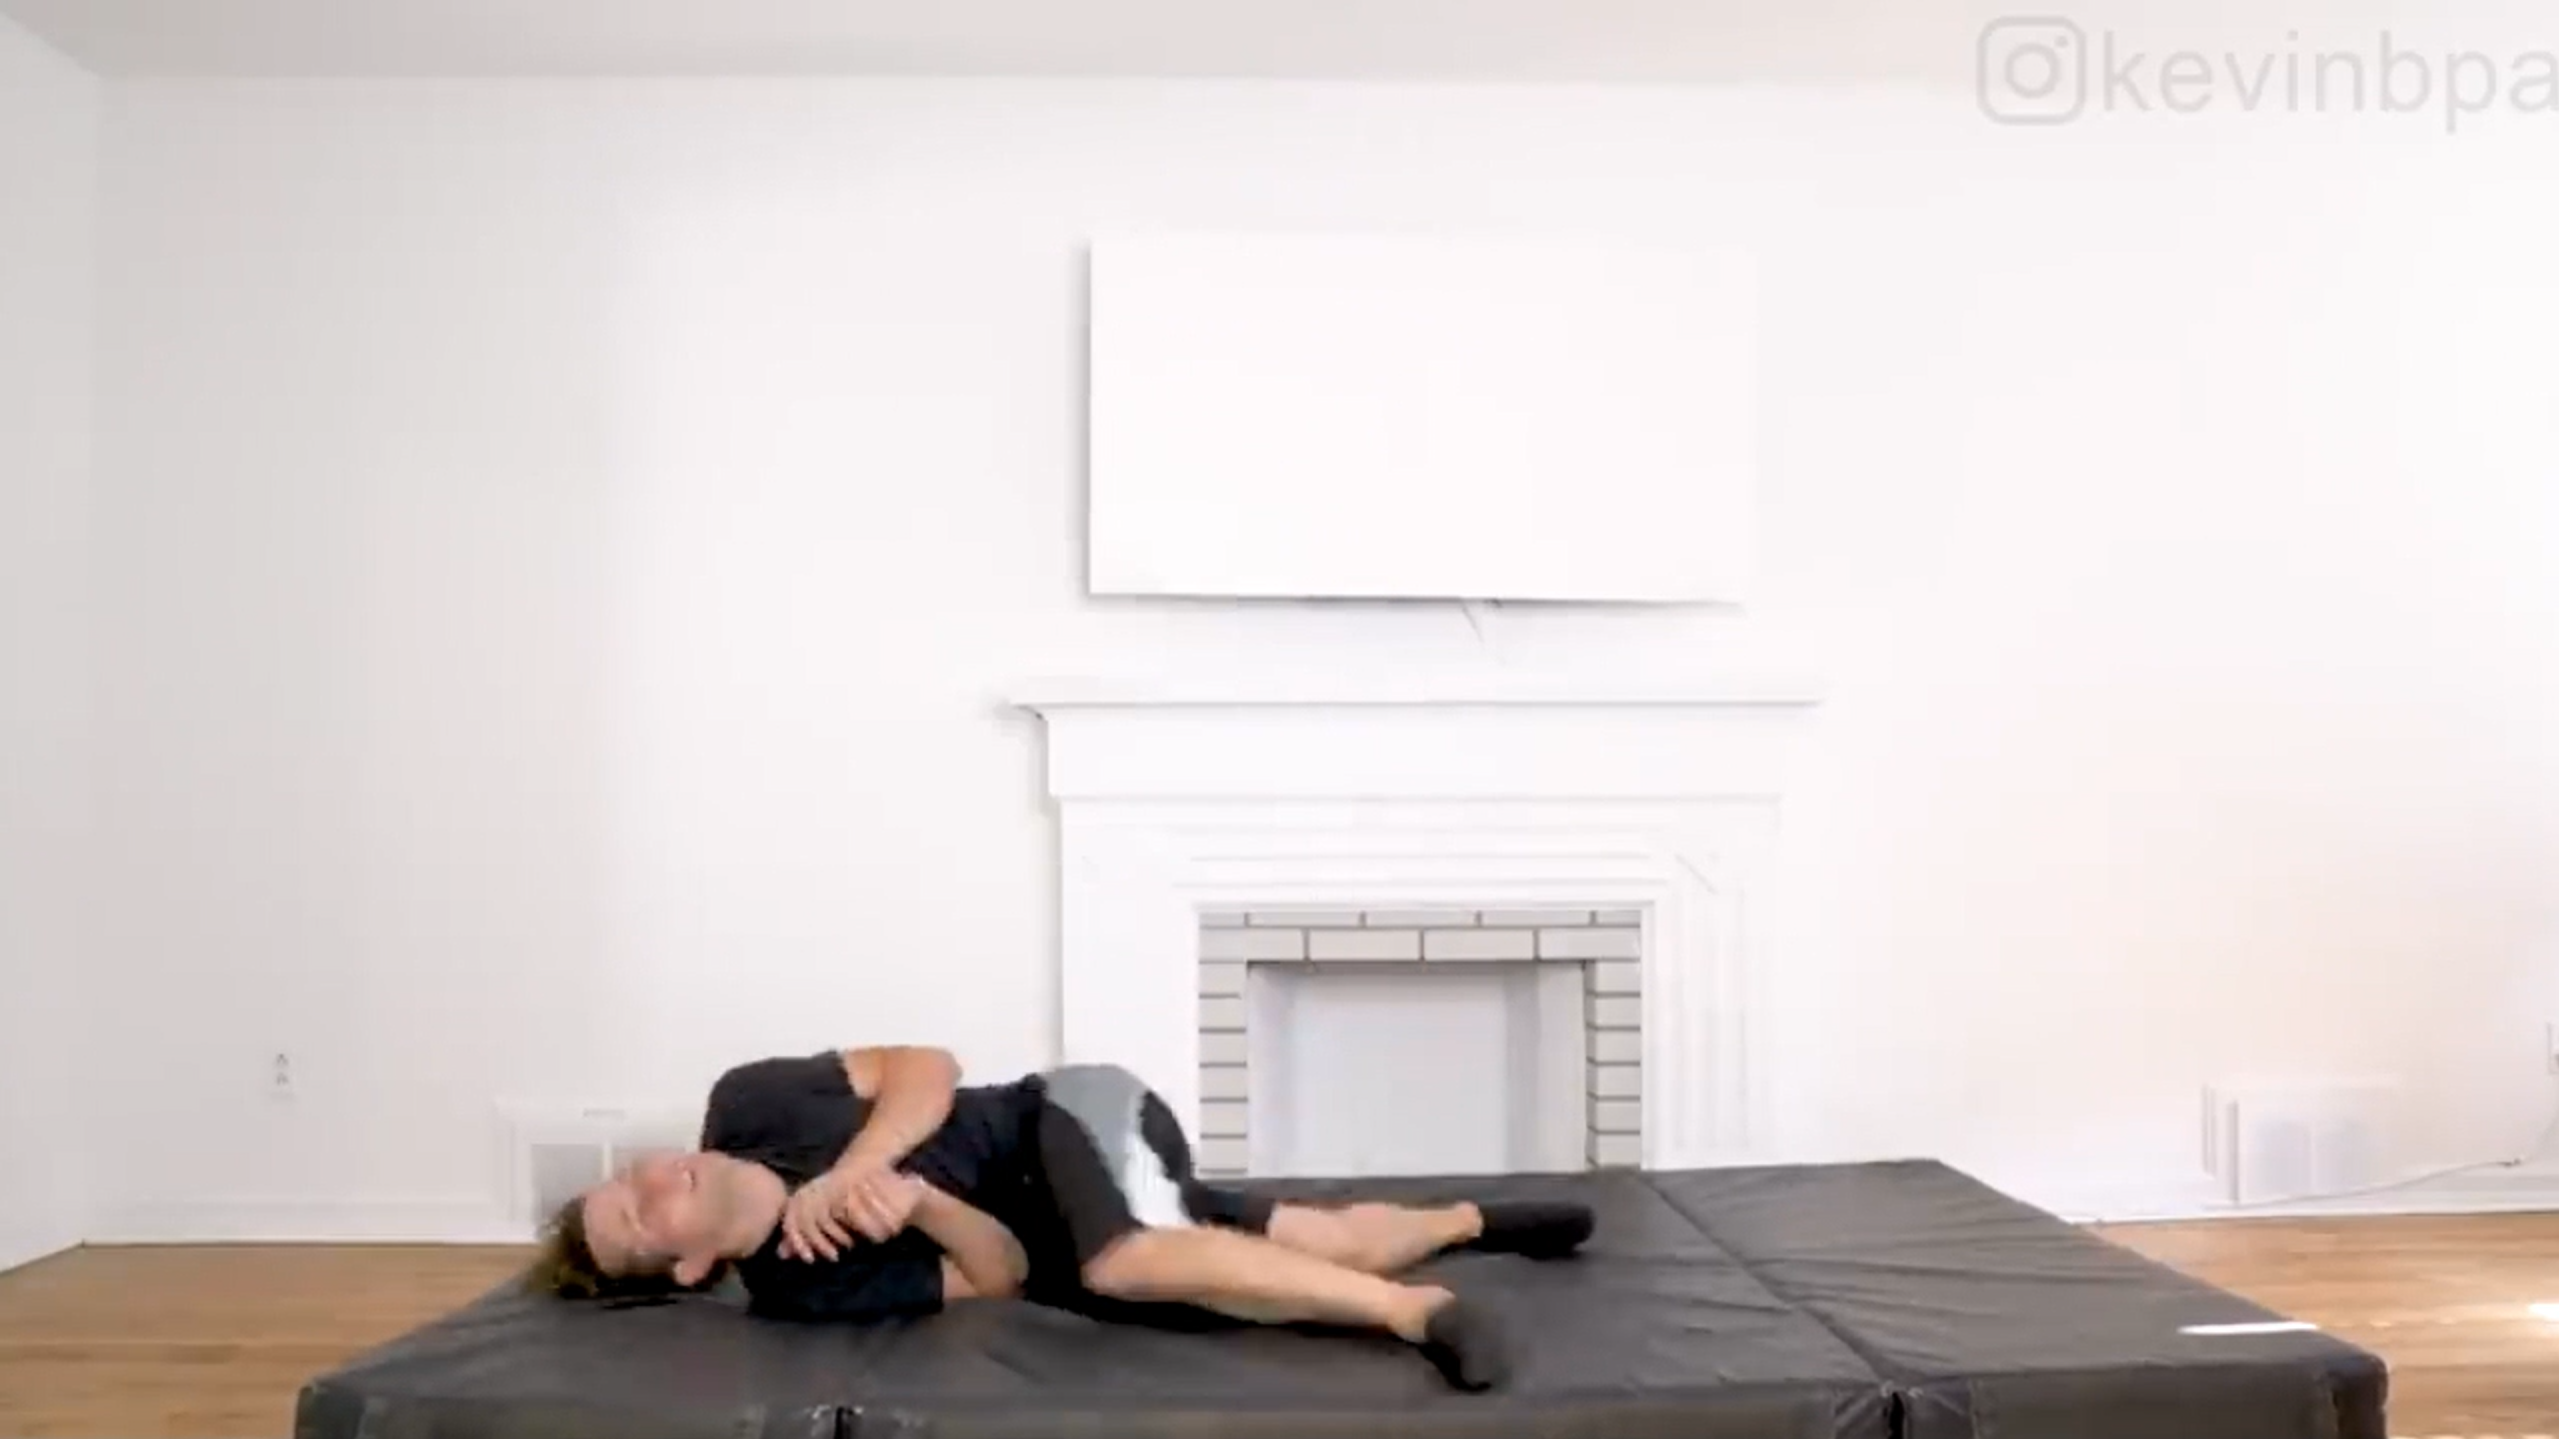
\includegraphics[width=0.45\textwidth]{Figures/datasets_examples/fifty2.png}
    \caption{Příkladové snímky z datasetů CAUCAFall (nahoře) a 50 Ways to Fall (dole).}
    \label{fig:datasets_examples}
\end{figure}

V obou případech se jedná o videa vždy jedné osoby. To proto, že použijeme
detekční algoritmus již natrénovaný na videích s více osobami, a náš
klasifikační algoritmus bude zpracovávat každou osobu zvlášť. Práce s více
osobami tak bude úlohou výsledného detektoru, nikoliv trénované klasifikační
sítě.

Videa z datasetu CAUCAFall jsou v rozlišení $720\times480$, zatímco videa z
datasetu 50 Ways to Fall jsou v rozlišení $1280\times720$.

Oba datasety byly rozděleny do tří sad: trénovací, validační a testovací.
Rozděleny byly v tomto poměru: trénovací sada 70\%, validační sada 15\% a
testovací sada 15\%. Trénovací a validační sada budou použity v procesu
trénování – trénovací pro výpočet ztráty a úpravu vah, validační pro průběžné
ověřování výkonu, testovací sada bude na konci použitá pro otestování jednak
klasifikačního algoritmu, jednak celkového řešení.

\section{Třídy a jejich anotace}
Pro videa byly vytvořeny anotace aktuální třídy pózy. Tato anotace není pro
každý snímek, ale pouze při změně definuje časovou značku a následující třídu.

V anotacích byly použity 3 třídy, ty odpovídají třem různým třídám pózy
relevantním k problému – \textit{normální}, kdy osoba např. chodí, sedí nebo
stojí, \textit{padá} – přechodný stav padání, definován od započetí pohybu
směrem dolů, a \textit{upadl} – definován od momentu, kdy se osoba dotkla země
trupem nebo všemi končetinami.

Pro řešený problém jsou obecně potřebné jenom dvě třídy – \textit{normální} a
\textit{upadl}. Skript tvořící trénovací data proto považuje třídu
\textit{padá} za třídu \textit{normální}. Nicméně do budoucna by se mohlo pro
pokročilejší optimalizaci zkusit experimentovat i se třídou \textit{padá},
která by mohla síti pomoct hlouběji pochopit problematiku a přesněji rozeznat
některé situace, zejména pak v případě využití rekurentních neuronových sítí.

\section{Příprava trénovacích dat pro klasifikační algoritmus}
\label{sec:TrainingDataPrep}

Dále byl vytvořen skript, který prošel každé video z trénovacích datasetů a na
základě výše zmíněných anotací vytvořil trénovací data pro klasifikační
síť. Ty obsahují pro každý snímek detekované klíčové body (jako vstup) a
aktuální třídu (jako požadovaný výstup). Pro detekci klíčových bodů byl použit
vybraný model pro detekci pózy. Výběr modelu je popsán v následující kapitole.
Na modelu použitém při tvorbě dat by teoreticky nemuselo záležet (pokud detekuje stejné typy
klíčových bodů), je ale lepší použít ve výsledném programu stejný model jako
pro trénovací data. Modely se totiž můžou v některých situacích chovat trochu
jinak (např. okluze) a klasifikační algoritmus by tak dostával v praxi jiná data, než pro
jaké byl natrénován.

Jelikož pro rekurentní neuronové sítě potřebujeme sekvenci snímků, musí být
trénovací data ještě zpracována. To ale bude již součastí samotného trénovacího
skriptu, jelikož se konečná podoba dat může lišit délkou sekvencí.
\endinput